%!TEX root = ../seminararbeit.tex
\section{Retrospektive bei \ac{sac}}\label{sec:retro}
\subsection{Retrospektive}
Im Team \textit{Modeling} werden in regelmäßigen Abständen Retrospektiven durchgeführt. 
Die Retrospektiven sind ein weiteres Konzept von Scrum. Sie haben das Ziel den vergangenen Sprint zu analysieren und aus den Fehlern zu lernen, aber auch  auf positive 
Geschehnisse hinzuweisen, um so das Team in Effizienz, Zusammenarbeit und Geimeinschaftsgefühl zu verbessern. \cite{retro:2018}. \\
Die Retrospektiven im \textit{Modeling} finden nicht nach jedem Sprint statt, sondern alle 6 Wochen.
\autoref{img:retroAblauf} zeigt den Ablauf einer Retrospektive. Je nach aktuellen Situationen können die 
verwendeten Methoden angepasst werden. Im Bezug auf die Thematik dieser Arbeit, Kriterien zur Ideenbewertung,  
sind besonders die Punkte \textit{Gewichtung der gefundenen Probleme} und \textit{Lösungsideen bewerten} relevant.

Die einzelnen Schritte erfüllen jeweils folgenden Zweck:
\begin{enumerate}
    \item In einer Retrospektive wird zunächst auf die letzte Retrospektive zurück geblickt. Es wird überprüft, ob die Ideen der letzten 
        Retrospektive umgesetzt wurden.
    \item Anschließend geht es darum neue Ideen für die nächsten 6 Wochen zu sammeln. Jedes Team-Mitglied
        hat die Möglichkeit positive und negative Geschehnisse vorzustellen.
    \item Die negativen Geschehnisse werden in Kategorien zusammengefasst. Dies ist die Vorgehensweise, die von Schawel-Billing vorgeschlagen wird.
    \item Als nächstes werden die negativen Kategorien bewertet. Ziel ist es, das schwerwiegendste Problem zu finden beziehungsweise 
    das Problem, dass die meisten verbessern möchten. Jedes Team-Mitglied kann hierzu eine Stimme abgeben. 
    \item Für die ausgewählte Kategorie müssen nun Lösungen gefunden werden. Jedes Teammitglied kann hierzu Ideen beisteuern. 
    \item Nun müssen die Ideen bewertet und konkrete Aufgaben an Team-Mitglieder verteilt werden.
\end{enumerate}
\begin{figure}[ht]
	\centering
	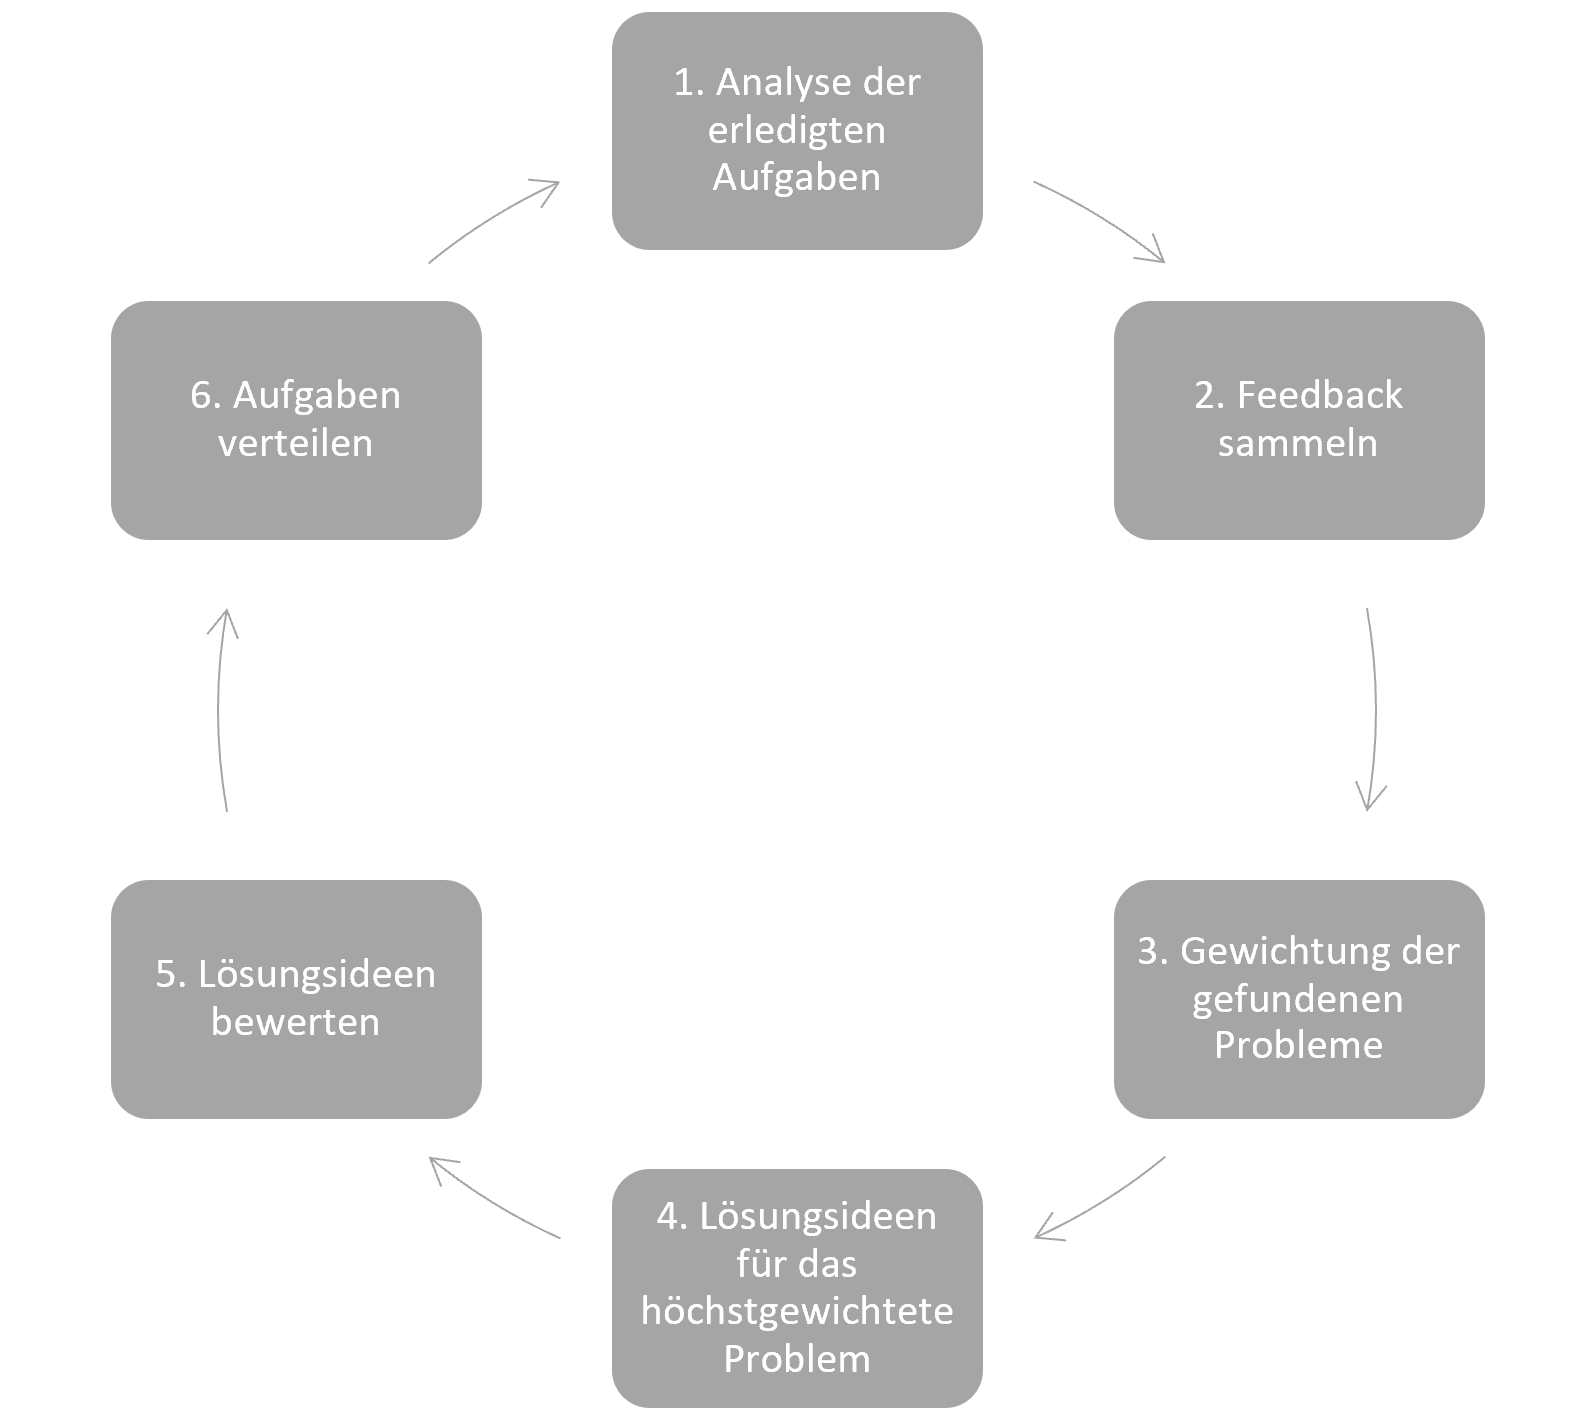
\includegraphics[width=10cm]{retroAblauf.png}
    \caption{Ablauf einer Retrospektive im Modeling}
	\label{img:retroAblauf}
\end{figure}
\subsection{Bewertung der Probleme}\label{sec:retro-punkte}
Für die Abstimmung darüber, welche Kategorie bearbeitet wird, zeigt sich die Methode \textit{Priorisierung mit Punkten} 
als geeignet. Auch Zephram schlägt dies als mögliche Bewertungsmethode vor.
\begin{quote}
    Die Grundidee ist die, dass jeder Teilnehmer eine gewisse Zahl an Stimmen (z.B. in Form von Klebepunkten [...]) bekommt, die er auf die generierten Ideen verteilen kann. \cite{dotmocracy:2011}
\end{quote} 
Dies ist eine schnelle Methode, die dennoch jeden einzelnen Teilnehmer berücksichtigt. Ziel der Problembewertung ist es, das Problem zu 
finden, das die meisten Team-Mitglieder beschäftigt. Dies bedeutet wiederum, dass hierbei nicht nach vorgegebenen Kriterien 
vorgegangen wird, sondern dass die individuellen und subjektiven Meinungen der Team-Mitglieder gefunden werden sollen. 
Kriterium der Ideenbewertung ist ausschließlich, dass jedes Teammitglied die eigene Meinung wiedergibt. Dies wird hier explizit erwähnt, 
da eine Gefahr dieser Methode beispielsweise der Herdentrieb sein kann. Das bedeutet, dass ein Team-Mitglied 
ein Problem wählt, da es bereits die meisten Punkte besitzt. So könnte es zu Ablehnungs- bzw. Annahmefehler des Problems kommen. \cite{derby:2012}\\
Ein weiteres implizites Kriterium ist, dass das Problem lösbar sein sollte. Dies ist eigentlich ein Teil der Ideenbewertung.
Dennoch wird ein Problem, das nicht gelöst werden kann, von den meisten Mitgliedern nicht gewählt. 

\subsection{Bewertungskriterien für Ideen}\label{sec:retro-kriterien}
Im Gegensatz zur Bewertung der Probleme, gibt es -wie von Zephram beschrieben- bei der Auswahl der Lösungsideen einige Randbedingungen
und Erfolgskriterien die beachtet werden müssen.

\paragraph{Randbedingungen}
\begin{enumerate}
    \item Die Lösungsidee, muss von Team-Mitgliedern umsetzbar sein. Das bedeutet es sollten keine Ideen gewählt werden, die ausschließlich von Mitarbeitern auserhalb des Teams
    umgesetzt werden können. Zum Beispiel kann das Problem, dass es keine Klimaanlage in den Büros gibt, lediglich an die zuständige Stelle weitergeleitet werden.
    Keine Team-Mitglied kann selbst die Idee, eine Klimaanlage einzubauen umsetzen. 
    \item Eine weitere Randbedingung ist, dass die Idee innerhalb der folgenden 6 Wochen umgesetzt werden kann. Zu Beginn der 
    nächsten Retrospektive wird das Ergebnis analysiert.
    \item Besonders wichtig ist, dass die Idee zur Lösung des Problems beiträgt. Oftmals ist es nicht möglich ein Problem vollständig zu lösen. 
    Deshalb sind Kompromisse möglich. Das Teammitglied, welches das Problem angesprochen hat, sollte diese Randbedingung bewerten. So 
    wird abgesichert, dass auch alle Teammitglieder das Problem richtig verstanden haben und so eine sinnvolle Lösung gewählt werden kann. 
\end{enumerate}

\paragraph{Erfolgskriterien}
\begin{enumerate}
    \item "Je schneller eine Idee zur Lösung des Problems führt, desto besser." 
    \item "Je effektiver eine Idee zur Lösung des Problems führt, desto besser."
    \item "Je mehr Mitarbeiter von der Lösung profitieren, desto besser."
\end{enumerate}

Das bedeutet zum einen, eine Abwägung zwischen Aufwand und Nutzen der Lösung und zum anderen sollten möglichst viele Mitarbeiter 
von der Lösung profitieren. Deshalb wird die Entscheidung über die Umsetzung eine Idee, im gesamten Team besprochen. 